\appendix

\section{Security and Privacy with Leaked $ID_U$}
\label{sp-leak-uid}
\usso\ requires $ID_U$ is known only to the honest IdP,
so a user inputs her username in the authentication to the IdP and $ID_U$ is processed only by the IdP internally.
$ID_u$ may be calculated by hashing a username concatenated with the IdP's secret key, or the IdP encrypts user identities in storage and decrypts them only in memory.

If some users' identities were leaked,
    colluding RPs could calculate $[ID_U]ID_{RP_j}$ for each known $ID_U$ and link them.
So RP unlinkability is broken in this case.
On the other hand, IdP-based login tracing is still prevented,
    because the IdP always knows user identities and the proof of privacy against IdP-based login tracing (i.e., Theorem \ref{thm-idp-untraceability}) holds in this case.

\subsection{Patched Step for Leaked $ID_U$}
In the case of leaked user identities,
RP designation and user identification are broken as below.
For example, in order to log into an honest RP as a victim user, whose account is $Acct' = [u']ID_{RP'}$,
    a malicious user with $ID_U = u$ randomly chooses $x$ in $\mathbb{Z}_n$,
    and colludes with some malicious RP to request an identity token by directly sending $PID_{RP} = [x^{-1}u^{-1}]Acct'$ to the IdP.
A token binding $PID_{RP} = [x^{-1}u^{-1}]Acct'$ and $PID_U = [u]PID_{RP} = [x^{-1}]Acct'$ will be signed by the IdP.
Then, the malicious user visits the honest RP using this token and the trapdoor $x$,
    and the derived account will be $[xx^{-1}]Acct'=Acct'$.
Or, after obtaining a token binding $PID_{RP} = [t]ID_{RP}$ and $PID_U = [u]PID_{RP}$,
    this malicious user could impersonate the victim at the designated honest RP
     using this token and the trapdoor $tu^{-1}u'$, and the derived account will be $[u']ID_{RP}$.

Therefore, in order to provide secure SSO services \emph{proactively} against this risk,
     in Step 4.2 an RP always calculates $PID_{RP} = [t]ID_{RP}$ by itself and
        accepts identity tokens only with matching $PID_{RP}$.
This patch keeps secure SSO services in \usso\ when user identities are leaked.

\subsection{Security Analysis}
\label{proof-rp-collision}

Assume $p$ RPs totally in \usso,
    whose identities are denoted as $\mathbb{ID}_{RP} = \{[r_{j; 1 \leq j \leq p}]G\}$.
We analyze that, in the case of leaked user identities,
    RP designation and user identification are ensured after the patch in Step 4.2 as described above.

\begin{lemma}[$PID_{RP}$ Collision-Freeness]
\emph{Given $\mathbb{ID}_{RP}$, an adversary cannot find $t$ and $t'$ satisfying $[t]ID_{RP_j} = [t']ID_{RP_{j'}}$ where $j \neq j'$.}\label{thm-rp-collision}
\end{lemma}

\noindent\textbf{\textsc{Proof.}} 
Finding $t$ and $t'$ that satisfy $[t]ID_{RP_j} = [t']ID_{RP_{j'}}$, can be described as a $PID_{RP}$-collision game $\mathcal{G}_C$ between an adversary and a challenger: the adversary receives from the challenger a finite set of RP identities, i.e., $ID_{RP_1}$, ..., $ID_{RP_p}$, and outputs $(a, b, t, t')$ where $a \neq b$. If $[t]ID_{RP_a}=[t']ID_{RP_b}$, which occurs with a probability ${\rm Pr}_s$, the adversary succeeds in this game.
%The attack success probability is defined as ${\rm Pr}_s$.

As depicted in Figure \ref{fig:ecdlp_algorithm}, we design a probabilistic polynomial time (PPT) algorithm $\mathcal{D}^*_C$ based on $\mathcal{G}_C$, to solve the ECDLP: find a number $x \in \mathbb{Z}_n$ satisfying $Q = [x]G$, where $Q$ is a point on $\mathbb{E}$ and $G$ is a generator on $\mathbb{E}$ of order $n$.

%where ${\rm Pr}\{\}$ denotes the probability.
%where $k$ denotes the security parameter and $\epsilon_{c}(k)$ becomes negligible when $k$ is sufficiently large.
%For any sufficiently large $k$, $m \ll 2^k$ since $m$ is a finite integer.

\begin{figure}[tb]
  \centering
  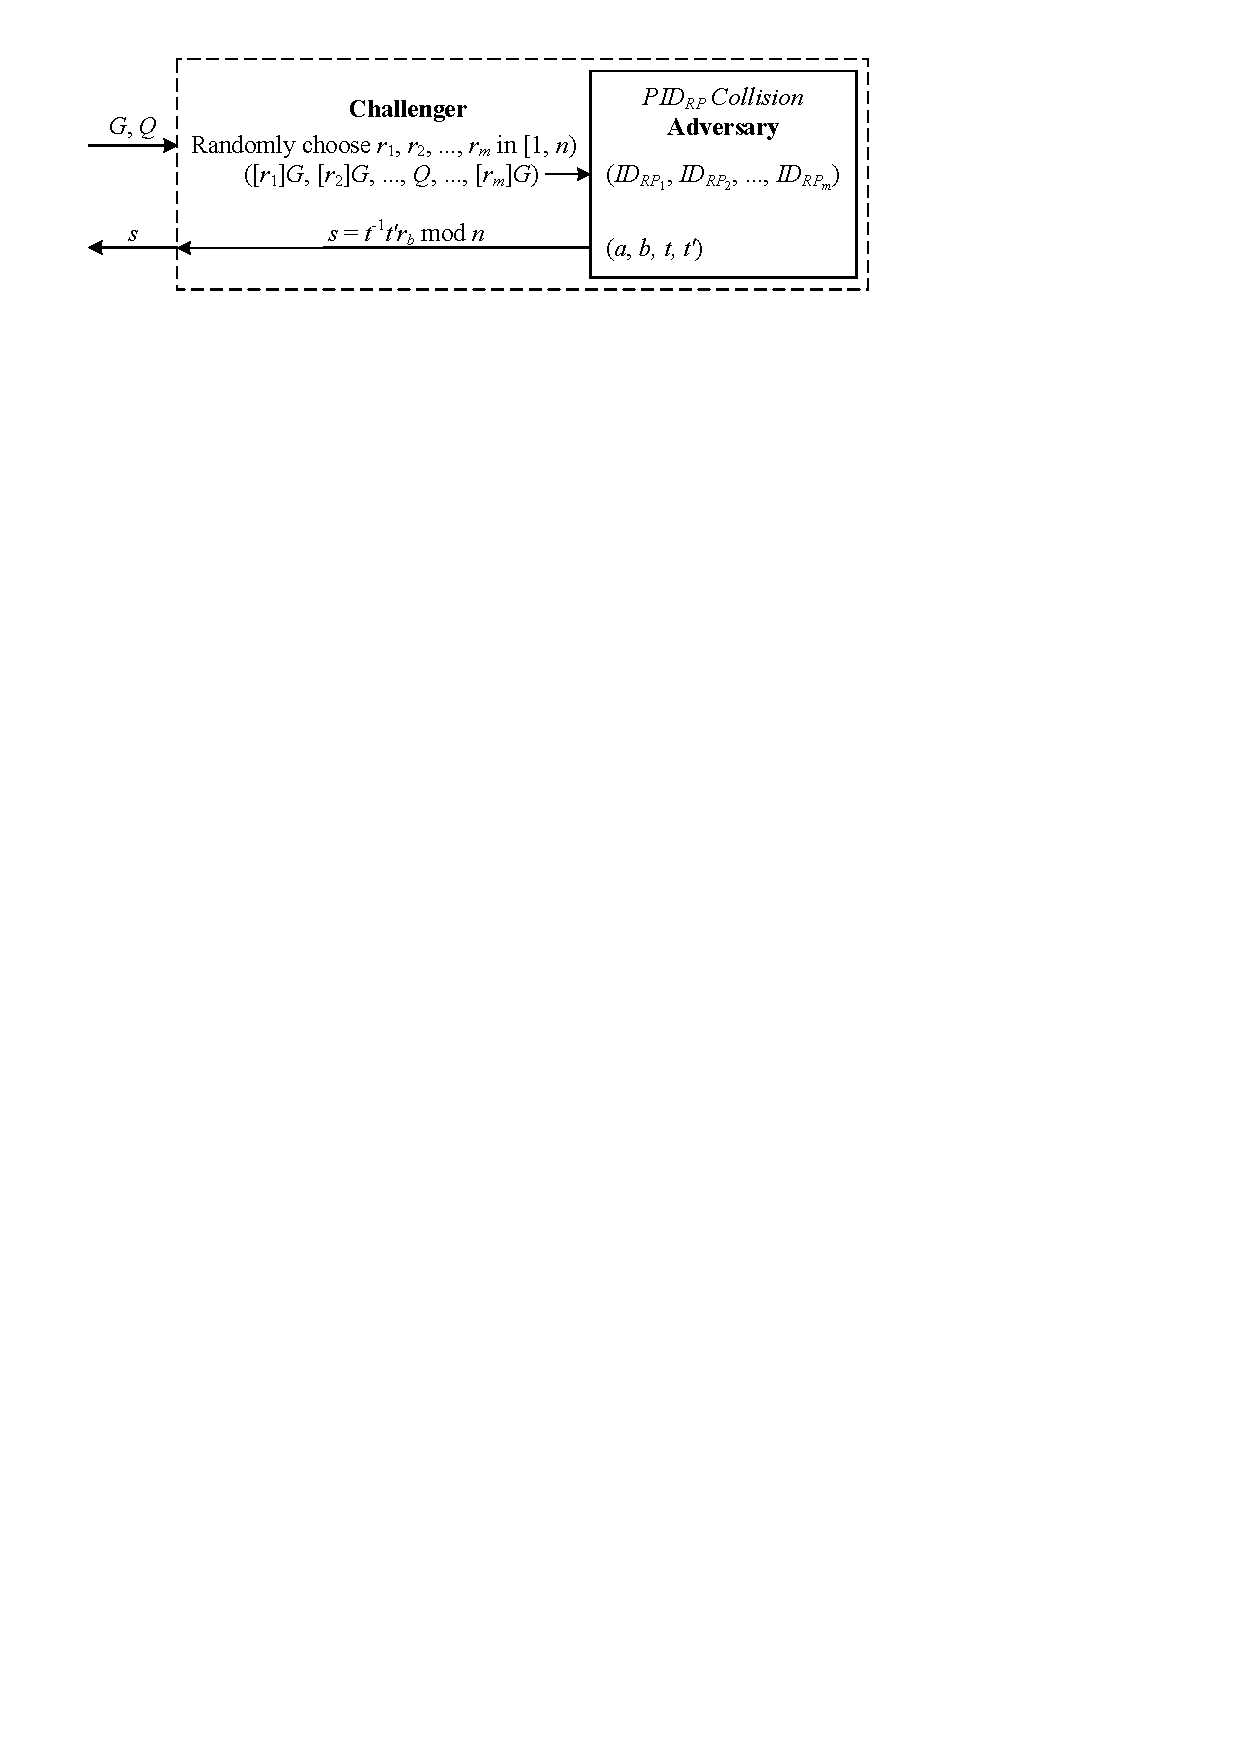
\includegraphics[width=0.96\linewidth]{fig/ecdlp_algorithm.pdf}
  \caption{The PPT algorithm $\mathcal{D}^*_C$ constructed based on the $PID_{RP}$ collision game to solve the ECDLP.}
  \label{fig:ecdlp_algorithm}
\end{figure}

The algorithm $\mathcal{D}^*_C$ works as below.
The input of $\mathcal{D}^*_C$ is in the form of ($G, Q$). On receiving an input ($G$, $Q$), the challenger first randomly chooses $r_1, \cdots, r_p$ in $\mathbb{Z}_n$ to calculate $[r_1]G, \cdots, [r_p]G$.
Then, it randomly chooses $j \in [1,p]$, replaces $[r_j]G$ with $Q$, and sends these $p$ RP identities to the adversary, which returns the result ($a$, $b$, $t$, $t'$).
Finally, the challenger calculates $e = t^{-1}t'r_b \bmod n$ and returns $e$ as the output of $\mathcal{D}^*_C$.

If the adversary succeeds in $\mathcal{G}_C$ and $[r_a]G$ happens to be replaced with $Q$, then $\mathcal{D}^*_C$ outputs $e=t^{-1}t'r_b =x$ because $[tr_a]G = [t]Q = [t'r_b]G$. For the adversary, $Q$ is indistinguishable from any other RP identities in the input set, as $[r_j]G$ is randomly replaced by the challenger.
Hence, the probability of solving the ECDLP using $\mathcal{D}^*_C$ is formulated as:
\begin{equation*}
{\rm Pr}\{\mathcal{D}^*_C(G, [x]G)=x\} = {\rm Pr}\{e = x\}={\rm Pr}\{a=j\}{\rm Pr}_s=\frac{1}{p}{\rm Pr}_s
\end{equation*}

If the probability of finding $t$ and $t'$ satisfying $[t]ID_{RP_j} = [t']ID_{RP_{j'}}$ is non-negligible, the adversary would have advantages  in $\mathcal{G}_C$ and ${\rm Pr}_s$ is non-negligible regardless of the security parameter $\lambda$.
Thus, we would find that ${\rm Pr}\{\mathcal{D}^*_C(G, [x]G)=x\}$ also becomes non-negligible even when $\lambda$ is sufficiently large, because $p$ is a finite integer and $p \ll 2^\lambda$.
This violates the ECDLP assumption. Therefore, the probability of finding $t$ and $t'$ that satisfy $[t]ID_{RP_j} = [t']ID_{RP_{j'}}$ is negligible.
\hfill $\square$
\vspace{.6mm}

\noindent \textbf{RP Designation.} 
Due to this collision-freeness property of $PID_{RP}$,
    an identity token designates \emph{only} the target RP and any other (honest) RP will reject this token.
So RP designation is ensured after the patch in Step 4.2, in the case of leaked user identities.

\noindent \textbf{User Identification.} 
Because $t$ is verified with $PID_{RP}$ and $ID_{RP}$ by the target RP,
 the only meaningful account derived
from $TK$ binding $PID_{RP}=[t]ID_{RP}$ and $PID_U = [u]PID_{RP}$,
 is exactly $[t]PID_U =[u]ID_{RP}$. Thus, user identification is also ensured.

